\documentclass[oneside,final,14pt]{extreport}

%% my command
%%%%%%%%%%%%%%
% Путь к файлу с изображениями
\newcommand{\picPath}{img}
% Величина отступа
\newcommand{\indentSpace}{1.25cm}
% Сокращения
\newcommand{\urlTitle}{ $-$ URL: }
%%%%%%%%%%%%%%%


% Изменяем шрифт
\usepackage{fontspec}
\setmainfont{Times New Roman}
\listfiles

% Полуторный интервал
\linespread{1.6}

% Отступ
\setlength\parindent{\indentSpace}

% Математика
\usepackage{mathtools}


% Картинки
\usepackage{graphicx}
\usepackage{subcaption}

% Языковой пакет
\usepackage[russianb]{babel}

% Таблицы
\usepackage{tabularx}

% Настройка подписей к фигурам
% Меняем заголовки картинок
\usepackage[ labelsep= endash]{caption}
\captionsetup{%
   figurename= Рисунок,
   tablename= Таблица,
   justification= centering% Формат - по центру
}         

% Кирилица в подфигурах
\renewcommand{\thesubfigure}{\asbuk{subfigure}}
% разделитель в подфигурах - правая скобка
\DeclareCaptionLabelSeparator{r_paranthesis}{)\quad }
\captionsetup[subfigure]{labelformat=simple, labelsep=r_paranthesis}

% Добавляем итератор \asbuk,
% чтобы использовать кирилицу
% как маркеры
\usepackage{enumitem}
\makeatletter
\AddEnumerateCounter{\asbuk}{\russian@alph}{щ}
\makeatother

% Меняем маркеры в перечислениях
% Списки уровня 1
\setlist[enumerate,1]{label=\arabic*),ref=\arabic*}
% Списки уровня 2
\setlist[enumerate,2]{label=\asbuk*),ref=\asbuk*}
% Перечисления
\setlist[itemize,1]{label=$-$}
% Удаляем отступы перед и после
% списка
\setlist[itemize]{noitemsep, topsep=0pt}
\setlist[enumerate]{noitemsep, topsep=0pt}

% Красная строка в начале главы
\usepackage{indentfirst}

% Убиваем перенос
\usepackage[none]{hyphenat}

% Перенос длинных ссылок
\usepackage[hyphens]{url}
\urlstyle{same}

% Выравнивание по ширине
\usepackage{microtype}

%\usepackage[fontfamily=courier]{fancyvrb}
%\usepackage{verbatim}%     configurable verbatim
% \makeatletter
%  \def\verbatim@font{\normalfont\sffamily% select the font
%                     \let\do\do@noligs
%                     \verbatim@nolig@list}
%\makeatother

% Границы
\usepackage{vmargin}
\setpapersize{A4}
% отступы
%\setmarginsrb 
%{3cm} % левый
%{2cm} % верхний
%{1cm} % Правый
%{2cm} % Нижний
%{0pt}{0mm} % Высота - отступ верхнего колонтитула
%{0pt}{0mm} % Высота - отступ нижнего  колонтитула

\setlength\hoffset{0cm}
\setlength\voffset{0cm}
\usepackage[top=2cm, bottom=2cm, left=3cm, right=2cm,
]{geometry}
 		
% Настройка заглавиий
\addto\captionsrussian{% Replace "english" with the language you use
  \renewcommand{\contentsname}% содержания
    {\hfill\bfseries
    СОДЕРЖАНИЕ
	\hfill    
    }%
   \renewcommand{\bibname}% списка источников
    {\hfill\bfseries
    	СПИСОК ИСПОЛЬЗОВАННЫХ ИСТОЧНИКОВ
	\hfill
	}% 
}%\

%\renewcommand{\contentsname}{\hfill\bfseries СОДЕРЖАНИЕ \hfill} 

% Настройка  заглавий в главах
\usepackage{titlesec}


%\titleformat
%{\chapter} % command
%[display]
%{
%\bfseries
%} % format
%{
%\thechapter.
%} 	% label
%{ 
%	0 pt
%} % sep
%{    
%\centering
%} % before-code

\titleformat{\chapter}
            {\bfseries}
            {\hspace{\indentSpace}\thechapter\hspace{1em}}
            {0pt}
            {
            \vspace{0mm} }
            [\vspace{14pt}]% Отступ после
% Начальный сдвиг заголовка 50 pt = 1.763888888cm.
% Второй параметр- сдвиг до = 2cm - 50pt
\titlespacing{\chapter}{0pt}{-0.2361cm}{0pt}

\titleformat{\section}
{\bfseries}{\hspace{\indentSpace}\thesection}{1em}{}

\titleformat{\subsection}
{\bfseries}{\hspace{\indentSpace}\thesubsection}{1em}{}

%\titleformat{\section}
%            {\bfseries}
%            {\thechapter.\hspace{1em}}
%            {0pt}
%            {\centering
%            \vspace{0mm} }
%            [\vspace{14pt}]% Отступ после
%\titlespacing{\section}{0pt}{-50pt}{0pt}

% Конец настройка заглавий

% Форматирование списка источников
\makeatletter
\renewcommand*{\@biblabel}[1]{\hfill#1}
\makeatother

% Убрать отсупы в списке источников
\usepackage{lipsum}

% ADD THE FOLLOWING COUPLE LINES INTO YOUR PREAMBLE
\let\OLDthebibliography\thebibliography
\renewcommand\thebibliography[1]{
  \OLDthebibliography{#1}
  \setlength{\parskip}{0pt}
  \setlength{\itemsep}{0pt plus 0.3ex}
}



% Добавить точки в оглавление
\usepackage{tocstyle}
\newcommand{\autodot}{.}


% Чтобы картинки вставляись
% куда надо
\usepackage{float}

% Для вычисления кол-ва страниц
\usepackage{lastpage}

% Для вычисления кол-ва рисунков и таблиц
%%%
\usepackage{etoolbox}

\newcounter{totfigures}
\newcounter{tottables}

\providecommand\totfig{} 
\providecommand\tottab{}

\makeatletter
\AtEndDocument{%
  \addtocounter{totfigures}{\value{figure}}%
  \addtocounter{tottables}{\value{table}}%
  \immediate\write\@mainaux{%
    \string\gdef\string\totfig{\number\value{totfigures}}%
    \string\gdef\string\tottab{\number\value{tottables}}%
  }%
}
\makeatother

\pretocmd{\chapter}{\addtocounter{totfigures}{\value{figure}}\setcounter{figure}{0}}{}{}
\pretocmd{\chapter}{\addtocounter{tottables}{\value{table}}\setcounter{table}{0}}{}{}
%%%

% Режим релиза
\sloppy
\usepackage{layout}

%\renewcommand{\arraystretch}{1.6}

\newcommand{\cmmnt}[1]{\ignorespaces}
\newcommand{\bs}{\boldsymbol}
\usepackage{breqn}
\begin{document}
\begin{center}
\bfseries РЕФЕРАТ
\end{center}

Дипломная работа содержит \pageref{LastPage} страниц, \totfig\ рисунков, \tottab\ таблицы, 5 источников.

МОБИЛЬНЫЙ РОБОТ, КОЛЕСО ИЛОНА, ОМНИ КОЛЕСО, ВИРТУАЛЬНОЕ ТЕСТИРОВАНИЕ РОБОТОВ, ROS, GAZEBO

Объектом исследования являются мобильные роботы, использующие роликонесущие колеса и методы управления ими.

Цель курсовой работы $-$ разработка конфигурации и алгоритма движения голономной роботизированной тележки.

В результате работы были разработаны кинематическая и динамическая модели мобильных роботов, использующих роликонесущие колеса для движения. Разработана компьютерная модель трехколесного мобильного робота, на основе которой протестирована кинематическая модель поведения голономного робота.

\tableofcontents
\newpage
\begin{center}
\bfseries ВВЕДЕНИЕ
\end{center}
\addcontentsline{toc}{chapter}{Введение}

Перед автором была поставлена задача $-$ исследовать виды движущихся роботизированных систем и методы управления ими. Особенный интерес изучения представляют роботизированные системы, использующие для передвижения роликонесущие колеса. Этот тип колес широко используется при создании роботизированных систем и позволяет роботам двигаться в любом заданном направлении в плоскости движения. Это увеличивает область применения роботизированных систем: в малых помещениях, в которых роботизированным системам на обычных колесах не хватает места для передвижения, роботы на роликонесущих колесах способны передвигаться без каких-либо ограничений. 

В процессе выполнения дипломной работы были разработаны модель роликонесущего колеса, механическая и кинематичесая модели тележек, опирающихся на $N$ роликонесущих колес, $N>2$, изучены и обозрены методы управления роботизированными системами. Полученные сведения протестированы на виртуальной модели робота с учетом всех физических сил, воздействующих на систему.

\chapter{Классификация мобильных роботов}
Мобильным роботом называют робота, способного менять свое местоположение в пространстве. Мобильные роботы могут быть автономными или управляемыми вручную. Автономные мобильные роботы способны без участия человека, основываясь на показаниях установленных на нем сенсоров и датчиков, определять свое местоположение и окружение, в котором они находится. Управляемый вручную робот не имеет такую возможность и способен передвигаться только по заранее заданной траектории.

Мобильные роботизированные системы подразделяются на голономные и неголономные. Мобильная роботизированная система называется голономной, если количество степеней свободы, доступных для управления, равно общему количеству степеней свободы системы. Иначе система называется неголономной[]. Характеристика голономности робота напрямую зависит от конфигурации механизма, приводяещего его в движение.
 
Для того, чтобы передвигаться в пространстве, мобильный робот должен иметь в своем устройстве механизм, приводящий его в движение. Мобильные роботы способны передвигаться используя следующие техники:
\begin{itemize}
\item ходьба;
\item прыжки;
\item скольжение;
\item качение;
\item плавание;
\item полет;
\item кувырки.
\end{itemize}
[ссылка на книжку]
Естественно, техники могут комбинироваться. 
 В рамках работы исследуются механизмы, позволяющие роботу двигаться по твердым горизонтальным поверхностям в земной среде. Кроме того, ограничим возможные техники движения ходьбой и качением Существующие роботы, способные двигаться по горизонтальной плоскости, делятся на следующие категории:
\begin{itemize}
\item роботы, использующие ноги для движеня;
\item роботы, использующие колеса для движения;
\item роботы, использующие гусеницы для движения.
\end{itemize} 
\section{Роботы, использующие ноги для движения}
Способ движения существующих роботов, использующих ноги, во многом повторяет способы предевижения биологических существ. Роботы этого типа имеют больше степеней своботы в сравнении с колесными роботами, что делает их устройство гораздо сложнее.

По своей конфинурации роботы, использующие ноги, отличаются количеством используемых ног. Существуют одноногие роботы, распространненими являются шестиногие роботы. Вообще, количество используемых для построения робота ног не ограничено. 

Для того, чтобы робот был способен стоять на поверхности, при этом не балансируя посредством приложения сил, ему необходимо как минимум три ноги. Кроме того, центр тяжести такого робота должен находится внутри области, образуемой многоугольником, каждая из вершин которой совпадает с координатой ноги. Но для движения такого типа роботов, он должен быть способны передвигать конечностями. 

Имея в арсенале три ноги, роботу невозможно добиться статичесткого равновесия во время ходьбы. Минимальное количество ног, необходимое для движения и постоянного поддержания статического равновесия - шесть. В такой конфигурации существует способ движения конечностями, при котором робот всегда имеет три точки опоры. 

На практике, количество степеней свободы каждой ноги зависит от их общего количества. Так, каждой ноге шестиногого робота достаточно двух степеней свободы для движения. В то же время, двуногие роботы используют гораздо большее степеней свободы. Так, например, двуногий робот Atlas имеет 27 степеней свободы для перемещения. На рисунке \ref{Figure:LegRobots} изображены существующие решения роботов такого типа.


\begin{figure}[H]
  \centering
  \begin{subfigure}[b]{0.4\linewidth}
   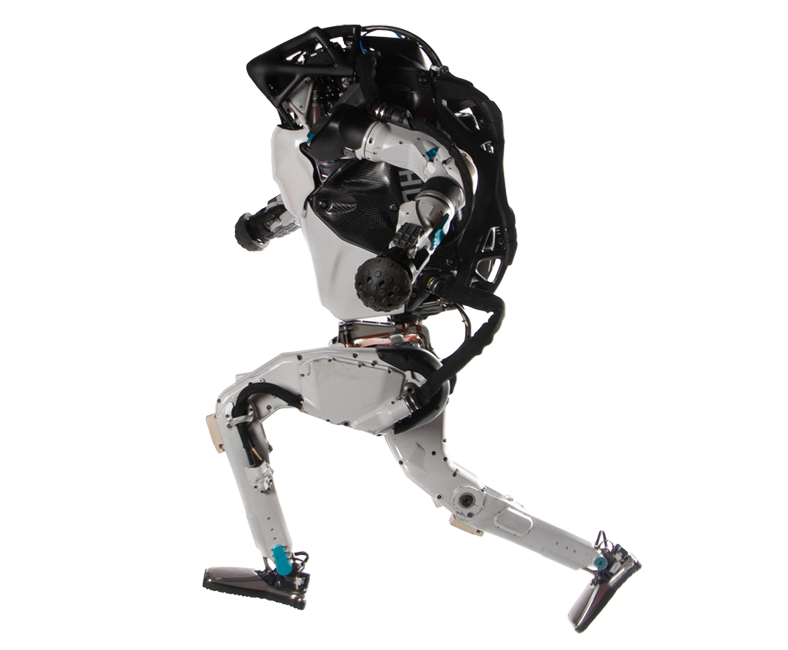
\includegraphics[width=\linewidth]{\picPath/LegRobots/atlas.png}
    \caption{ Двуногий робот Atlas компании Boston dynamics}
  \end{subfigure}
  \begin{subfigure}[b]{0.4\linewidth}
    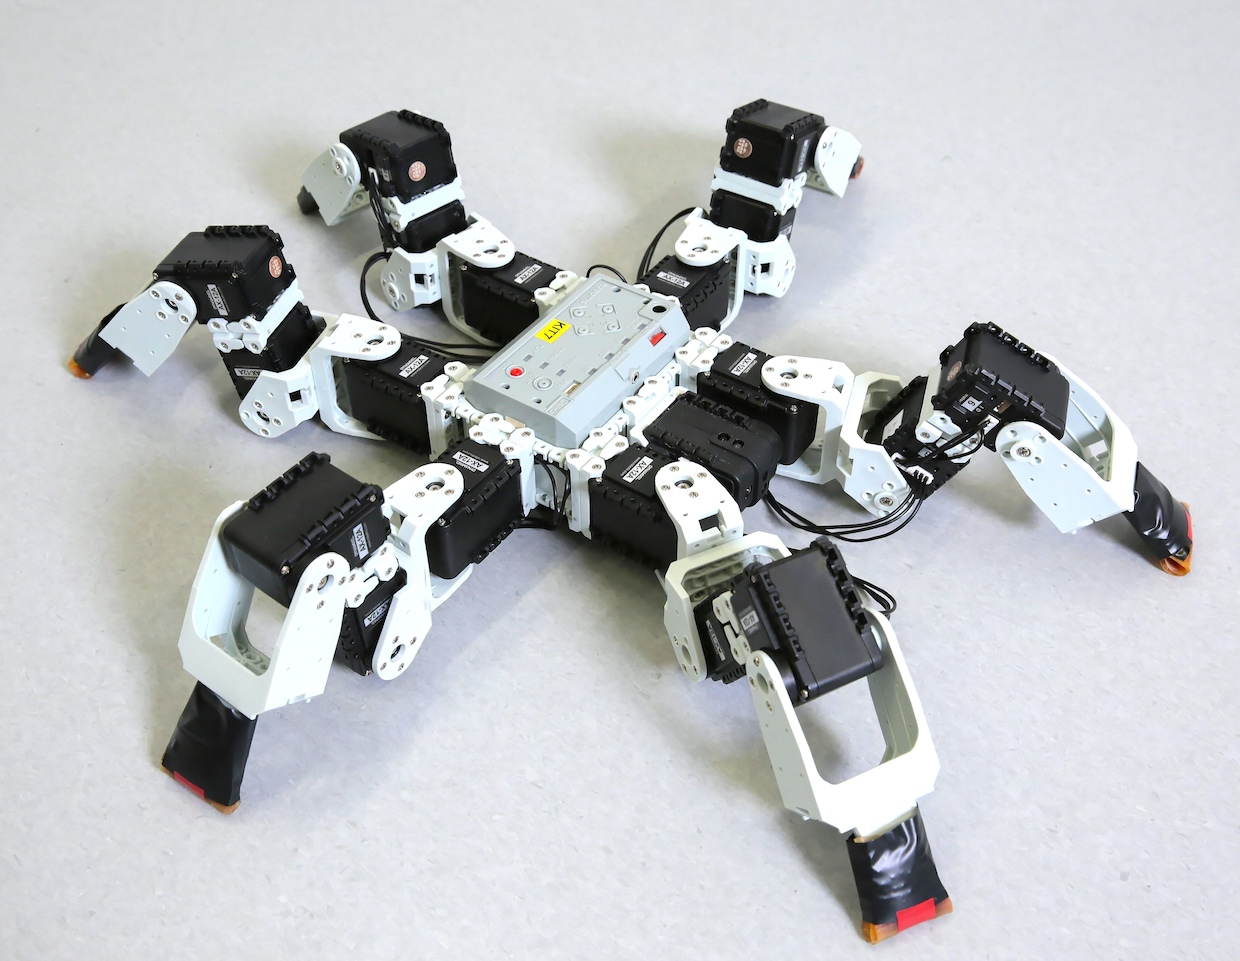
\includegraphics[width=\linewidth]{\picPath/LegRobots/sixLegRobot.jpeg}
    \caption{ Шестиногий робот, результат исследования[ссылка на источник]}
  \end{subfigure}
  \caption{ Современные роботы, использующие ноги для передвижения}
  \label{Figure:LegRobots}
\end{figure}
Основная характеристика роботов, использующих ноги, $-$ последовательность пятен контакта ног робота с поверхностью. Так как для движения такому роботу нужно всего несколько малых областей контакта, качество повехности не столь важно для его предвижения.

Роботы, использующие ноги, используются в условиях, когда поверхность движения не является плоской или материал поверхности мягкий. Во время качения по плоской твердой поверхности колесо имеет малую площадь соприкасновения с поверхностью, поэтому при качении колесо испытывает малое количество сопротивления. Неровности и мягкий материал поверхности увеличивает площадь поверхности колеса и уменьшает его эффективность. Для создания условий движения колеса требуется большое количество ограничений. Роботы, использующие ноги для движения, в отличие от колесных, имеют большую площадь соприкасновения с поверхностью, что дает им преимущество в сложных условиях.

Роботы, использующие ноги для движения, способны прередвигаться в сложных условиях, когда поверхность не является ровной, имеет подъемы или спуски или состоит из мягкого материала. Это позволяет широко использовать таких роботов в сложной среде. Кроме того, такие роботы способны преодолевать препядствия просто перешагивая их. К недостаткам роботов с ногами можно отнести высокую сложность механизма и сравнительно низкую скорость передвижения.
\section{Роботы, использующие колеса для движения}
Использование колес для передвижения - самый распространенный подход к построению мобильных роботов. Во время проектирования роботов, использующих ноги, много внимания уделятся проблеме их устойчивости, в то время как разработка колесных роботов практически лишена этой части проектирования. Несмотря на то, что для устойчивого положения робота в пространстве необходимо всего два колеса, большинство колесных мобильных роботов исплозуют три и более, что решает проблему устойчивости.

Основная задача, стоящая перед проектировщиками мобильных колесных роботов - маневриность и управляемость модели.

Как было описано выше, всякий мобильный робот может быть или голономным, или неголономным. Для случая колесных роботов это значит, что в любой момент времени робот может передвинуться в любом заданном направлении в плоскости. Так например стандартная конфигурация автомобиля не является голономной, в то время как тележка на роликонесущих колесах, описаная ниже, является.

На текущий момент существует множество типов конфигураций колес:
\begin{itemize}
\item обычное колесо;
\item роликовое колесо;
\item роликонесущее колесо.
\end{itemize}
\subsection{Обыкновенное колесо}
Обыкновенное колесо по своей сути $-$ диск или обод, вращающийся на оси или укреплённый на валу и служащий для приведения механизма в движение[словарь Ожигова].

Обычное колесо - самый распространненый тип колес, проподитель всех остальных типов, древнейшее изобретение человечества. Такие колеса повсеместно используются в автомобилях, поездах, самолетах и так далее. 

Для того, чтобы вычислить скорость центра колеса в условиях механики сплошных сред, необхоидимо знать его угловую скорость $\bs{\omega}$, радиус вектор некоторой точки границы диска $\bs{r}$ и скорость точки касания с поверхностью $\bs{V_{0}}$.

Если считать, что скорость поверхности движения равна нулю, то в случае, если верктор скорости $\bs{V_{0}}$ отличен от нуля, колесо скользит по поверхности. 

Тогда скорость центра колеса $\bs{V_{c}}$ будет равна

\begin{equation}
\bs{V_{c}}
=
\bs{V_{0}}
+
\bs{\omega}
\times
\bs{r}
\label{Equation:wheelSpeed}
\end{equation}

Обычное колесо широко используется и в робототехнике. На рисунке \ref{Figure:myCar} изображен робот-шпион, использующий обыкновенные колеса. 

Из-за того, что  колесо способно катить колесную тележку только в направлении, перпендикулярном оси его вращения, построение голономного робота, используеющего обыкновенные колеса, затруднительно. Для того, чтобы колесный робот на обычных колесах был способен менять направление движения, необходимо менять угол оси его вращения. Так, например, в стандартной конфигурации автомобиля передние оси вращения колес механически соеденины с рулевой рейкой, что позволяет маневрировать во время движения.  
\begin{figure}[H]
\begin{center}
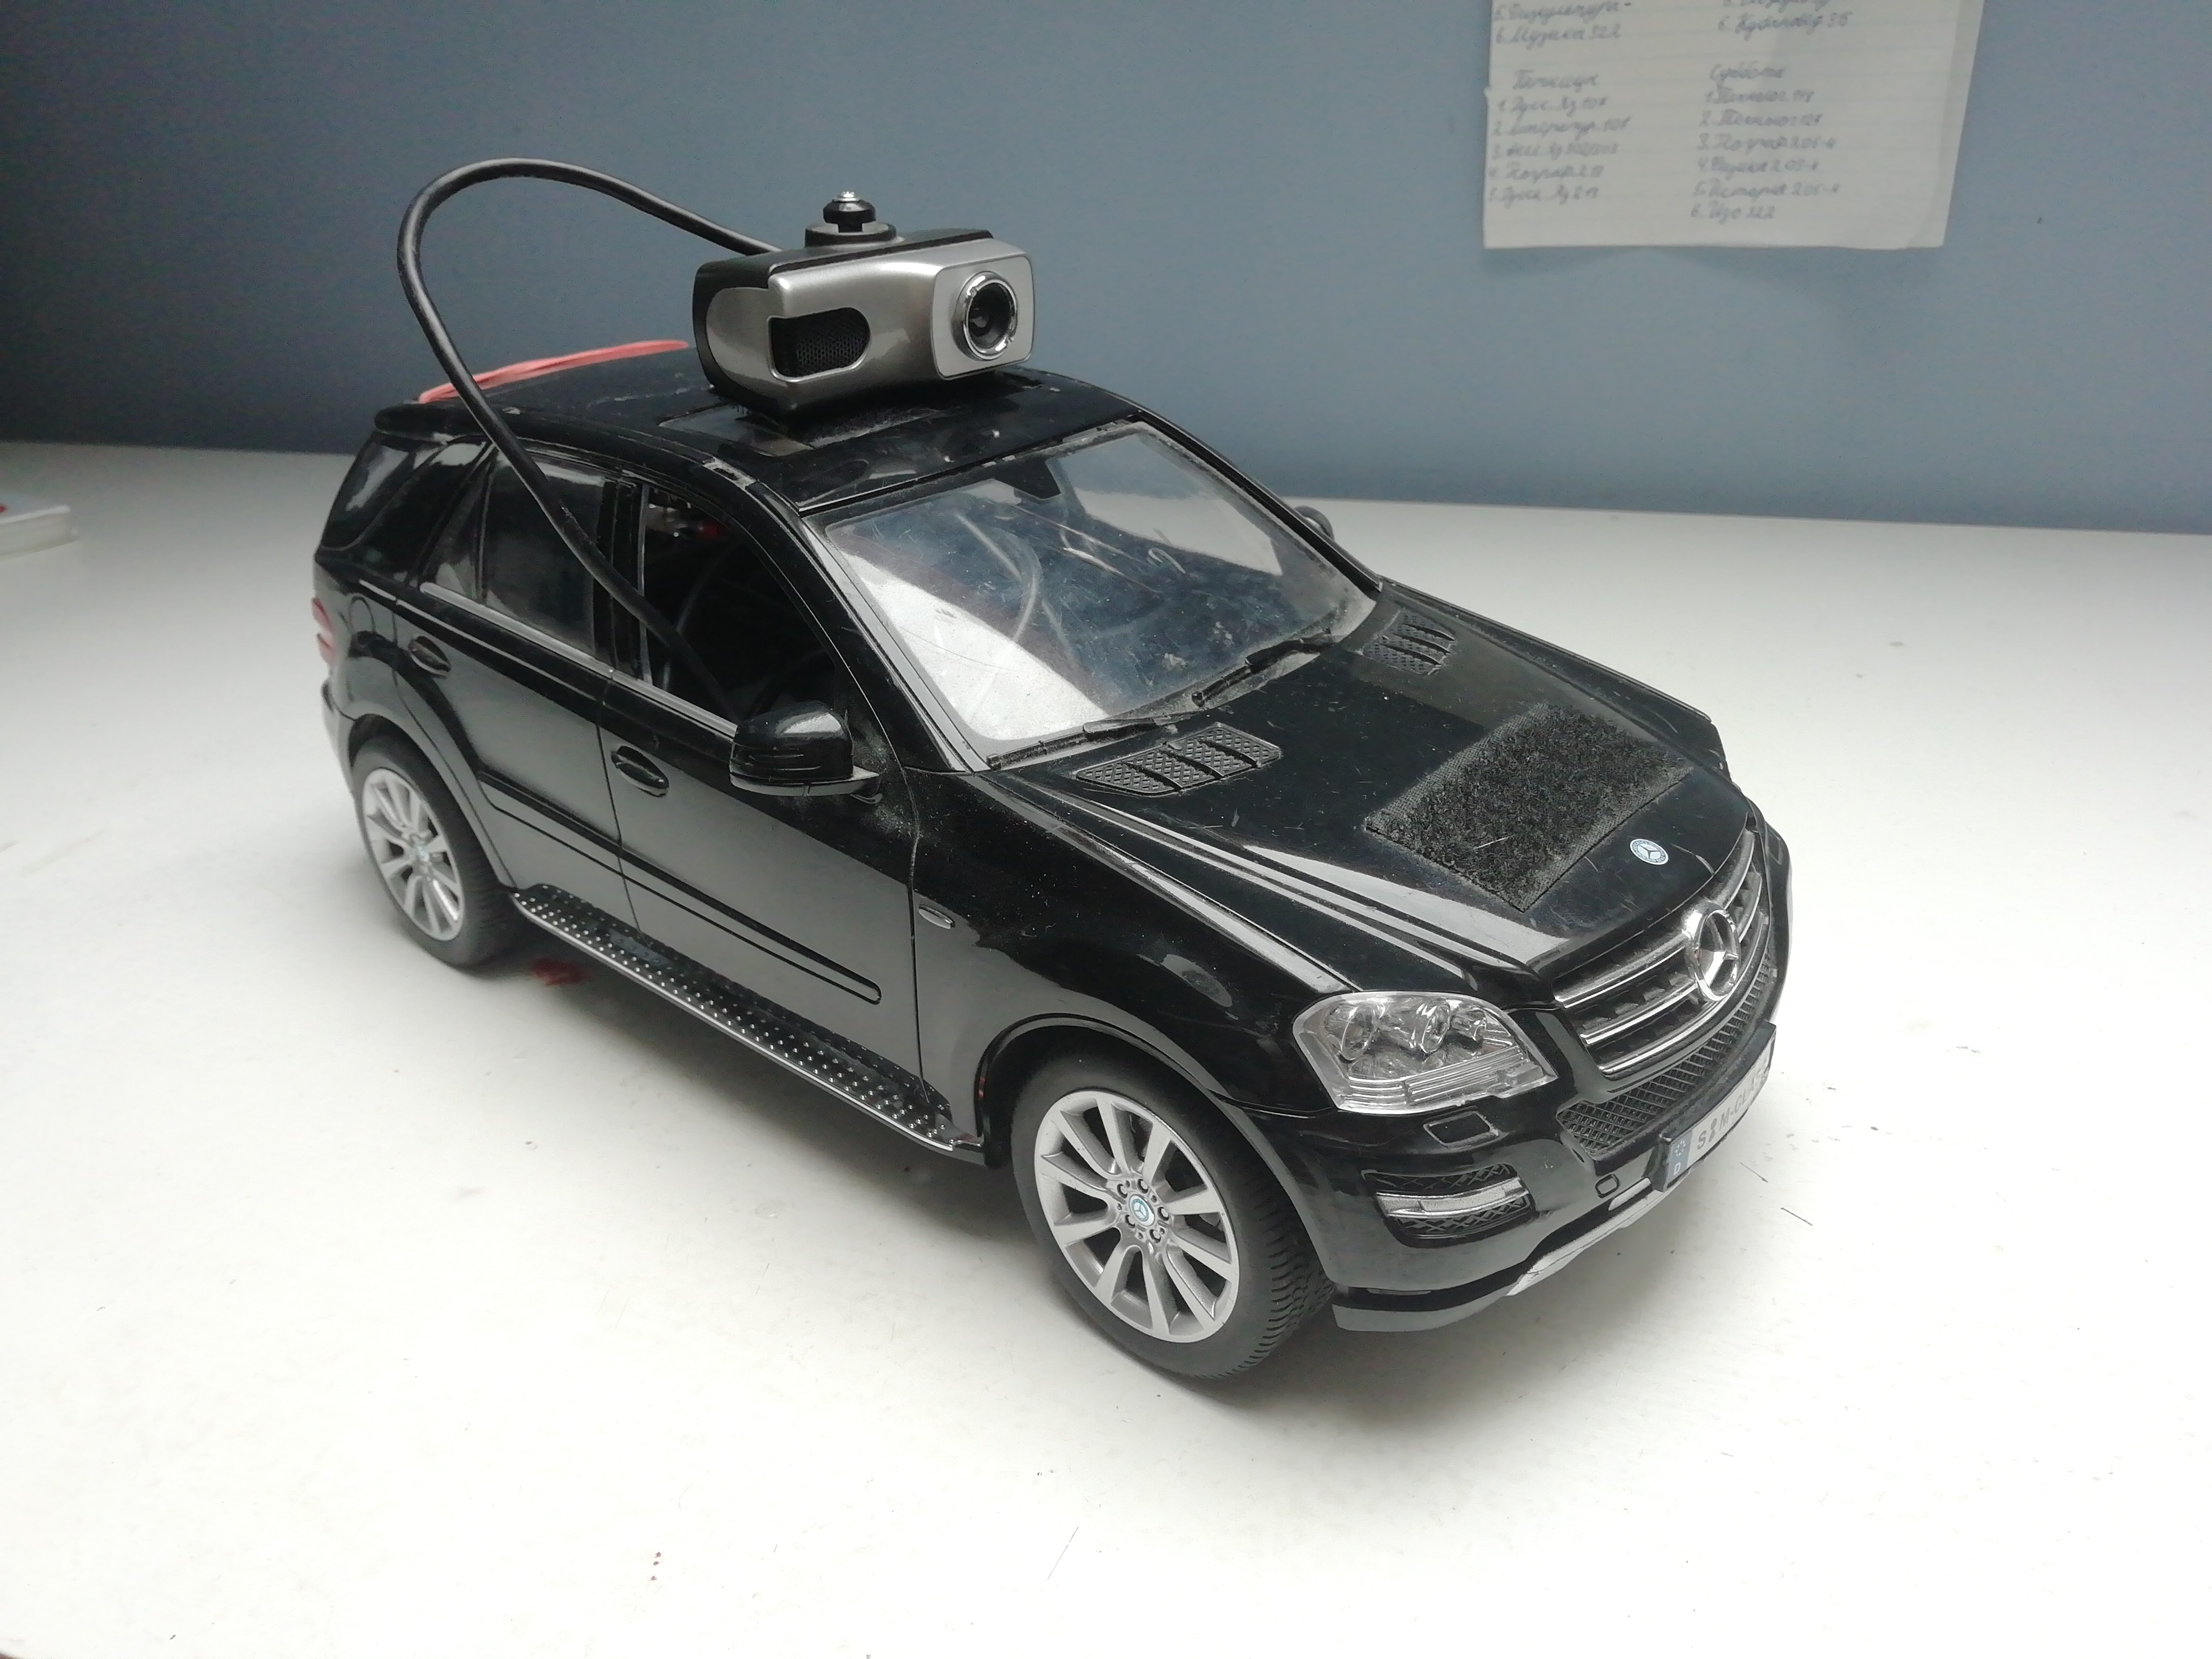
\includegraphics[width=0.5\linewidth]{\picPath/Cars/myCar.jpg}
\end{center}
  \caption{ Робот-шпион, использующий обычные колеса}
  \label{Figure:myCar}
\end{figure}
Главное достоинство обычного колеса - простота конструкции и минимальное трение качения в сравнении другими типами колес. К недостаткам относится тот факт, что обычное колесо имеет всего одну степень свободы. \cmmnt{движение обычного колеса возможно только в направлениях, перпендикулярных оси вращения.}
\subsection{Колесо castor wheel}
Castor wheel - распространенный тип колес, повсеместо используемый в каталках, продуктовых тележках, мебели и так далее. У этого типа колес нет определенного русского наименования; будем называть такие колеса роликовыми. Примеры роликовых колес изображены на рисунке \ref{Figure:CastorsWheels}.

Главное отличие роликового колеса от обычного - дополнительная степень свободы. Ось вращения такого колеса может вращается на $360$ градусов. Также, к таким колесам относят закрепленные шарики, способные катиться в любом направлении. 

\begin{figure}[H]
  \centering
  \begin{subfigure}[b]{0.4\linewidth}
   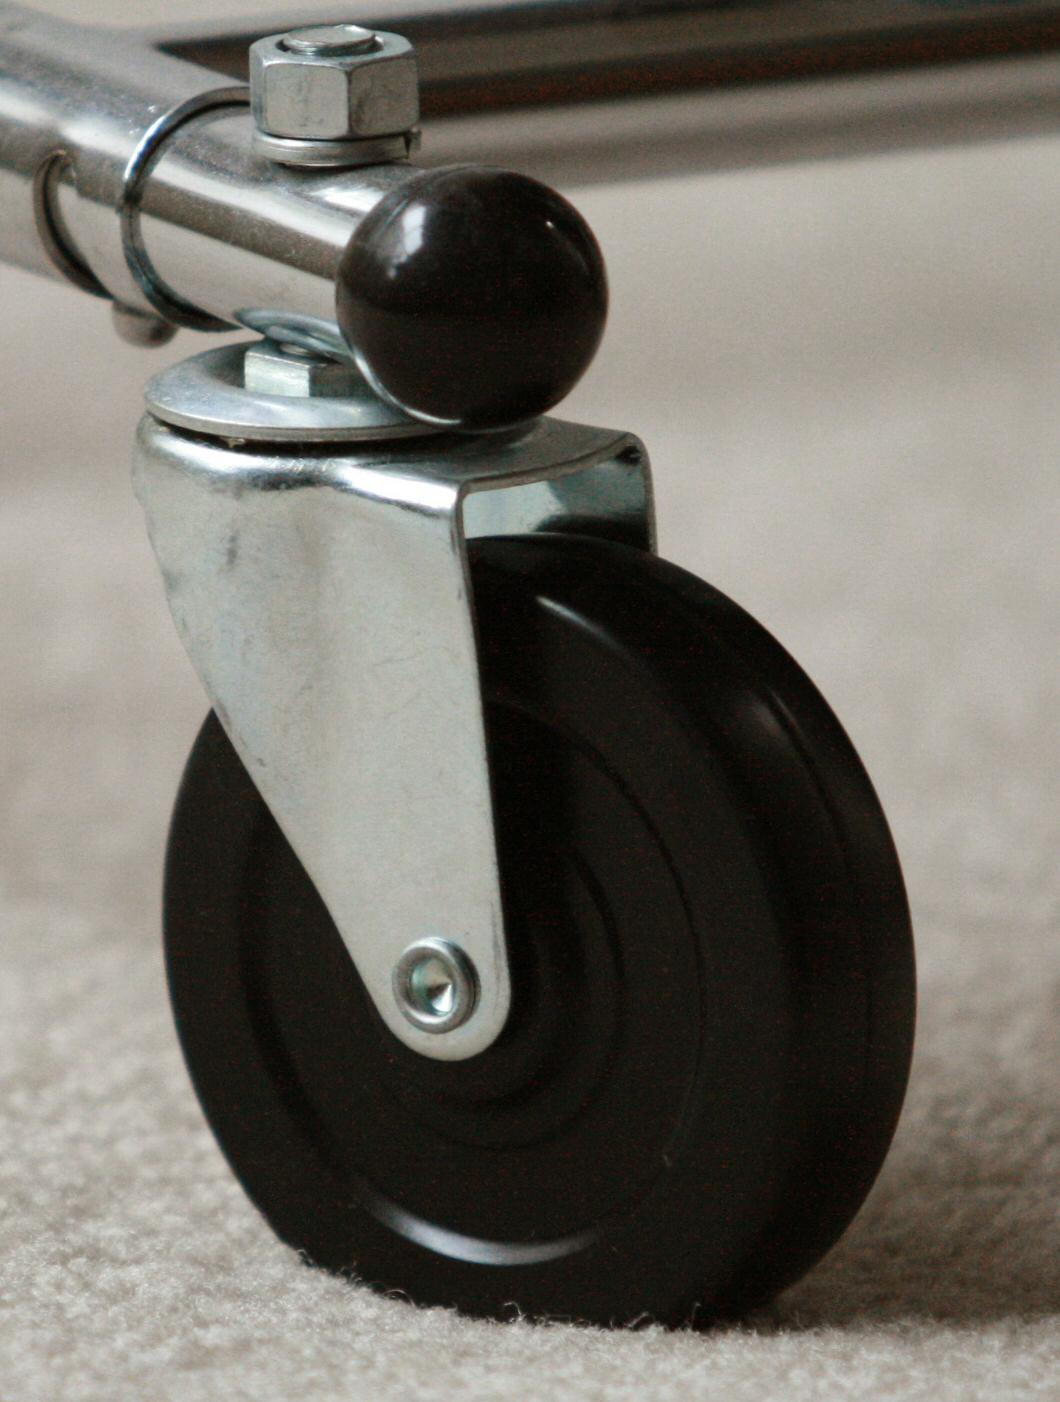
\includegraphics[width=\linewidth]{\picPath/Wheels/castorWheel.jpg}
    \caption{ Роликовое колесо тележки}
  \end{subfigure}
  \begin{subfigure}[b]{0.4\linewidth}
    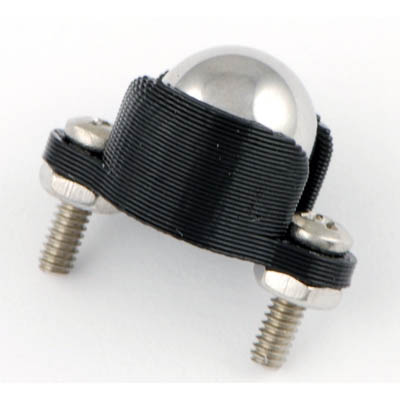
\includegraphics[width=\linewidth]{\picPath/Wheels/simpleBallWeel.jpg}
    \caption{ Шаровое колесо }
  \end{subfigure}
  \caption{ Роликовые колеса}
  \label{Figure:CastorsWheels}
\end{figure}
Благодаря двум степеням свободы роликовые колеса способны катиться в любом направлении. Однако из-за своей конструкции, привести само роликовое колесо в движение затруднительно. Роликовые колеса обычно используется для того, чтобы облегчить движение тяжелых объектов по поверхности, причем объекты приводятся в движения за счет внешних сил. В случае продуктовой тележки, силу для её движения прикладывает покупатель.


В робототехнике роликовые колеса широко используюся для увеличения маневренности. Распространненая конфигурация робота, использующего два обычных колеса и одно роликовое, изображена на рисунке \ref{Figure:threeWheelRobot}.
\begin{figure}[H]
\begin{center}
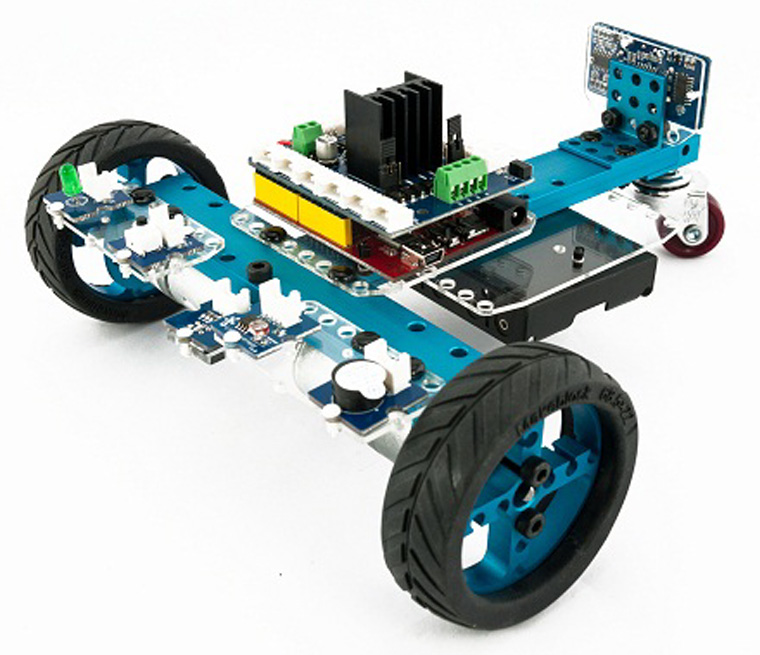
\includegraphics[width=0.4\linewidth]{\picPath/Cars/threeWheels.jpg}
\end{center}
  \caption{ Робот, использующий в своей конфигурации два обычных колеса и одно роликовое}
  \label{Figure:threeWheelRobot}
\end{figure} 
Такая конфигурация позволяет значительно увеличить маневренность робота. Приводя в движение одно из двух колес, тележка вращается на месте, описывая круги вокруг точки касания статичного колеса. Однако такая модель все-еще не является голономной. Движение строго перпендикулярно оси обычный колес все-еще невозможно.

\subsection{Роликонесущее колесо}
Роликонесущее колесо - колесо, имеющее на своем ободе ролики, каждый из которых вращающается вокруг собственной оси. Для примера распространенные виды роликонесущих колес изображены на рисунке \ref{Figure:rollerHandedWheels}.
\begin{figure}[H]
  \centering
  \begin{subfigure}[b]{0.4\linewidth}
   \includegraphics[width=\linewidth]{\picPath/Wheels/mecanumWheel.jpg}
    \caption{ колесо Илона }
  \end{subfigure}
  \begin{subfigure}[b]{0.4\linewidth}
    \includegraphics[width=\linewidth]{\picPath/Wheels/omniWheel.jpg}
    \caption{ омни колесо }
  \end{subfigure}
  \caption{ Роликонесущие колеса}
  \label{Figure:rollerHandedWheels}
\end{figure}
Главная характеристика роликонесущего колеса - угол между осью вращения колеса и  осью ролика, касающегося поверхности вращения ролика $\alpha$. Благодаря вращению роликов, скорость точки касания с поверхностью $\bs{V_{0}}$ из выражения \ref{Equation:wheelSpeed} не равна нулю. Роликонесущее колесо, во время движения, как-бы скользит на установленном на нем ролике в направлении, перпендикулярном оси этого ролика. Это позволяет роботам, использующим такие колеса для передвижения, двигаться в любом заданном направлении. Подробное математическое исследование этого явления описано в главе ...

Роликонесущее колесо относительно молодое изобретение. Первое упомнинание о нем относится к 1919 году[US patent 1305535], однако в том виде, в котором оно используется сегодня, такое колесо, названное омни колесом, появилось только в	1974 году[US patent 3789947]. Особенность омни колеса в том, что угол $\alpha = 90^{\circ}$, благодаря чему оно может свободно скользить в любом направлении.

8 апреля 1975 года шведский изобретатель Бенгт Ирланд Илон запотентовал свое изобретение - колесо Илона или, по названию компании, в которой он работал, Mecanum wheel[патент]. Инновация заключается в том, что   угол $\alpha$  лежит в пределах $30^{\circ}-60^{\circ}$  градусов, что позволяет устанавливать такие колеса паралельно друг-другу, и при этом не терять свойство голономности. На рисунке \ref{Figure:holonomicRobots} изображены роботы, использующие для движения роликонесущие колеса типа омни колесо и колесо Илона.


На рисунке \ref{Figure:mecanum_car_simple} изображена возможная конфигурация робота на колесах Илона. Так как угол $\alpha$ не прямой, то устанавливая колеса так, чтобы прямые, проходящие через оси касающихся поверхности роликов, попарно пересекались ($\bs{l_{2}}$,$\bs{l_{3}}$ и $\bs{l_{1}}$,$\bs{l_{4}}$), придем к выводу: вектора скорости точек касания колес с поверхностью не равны нулю и не паралельны. А это значит, изменяя длинну векторов скоростей, мы можем задать любое направление движения. В случае омни колеса, колеса не могут находиться паралельно друг-другу: для голономности необходимо, чтобы прямые, прходящие через оси роликов, пересекались. 

\begin{figure}[H]
\centering{
\resizebox{135mm}{!}{\input{mecanum_car_simple.pdf_tex}}
\caption{ модель тележки на четырех колесах Илона}
\label{Figure:mecanum_car_simple}
}
\end{figure}

\begin{figure}[H]
  \centering
  \begin{subfigure}[b]{0.4\linewidth}
   \includegraphics[width=\linewidth]{\picPath/Cars/mecanumWheel.jpg}
    \caption{ мобильный робот, движимый четырмя колесами Илона }
  \end{subfigure}
  \begin{subfigure}[b]{0.4\linewidth}
    \includegraphics[width=\linewidth]{\picPath/Cars/omniWheel.jpg}
    \caption{ мобильный робот, движимый тремя омни колесами }
  \end{subfigure}
  \caption{ Голономные мобильные роботы компании Nexus robot}
  \label{Figure:holonomicRobots}
\end{figure}
Выбор между углом наколна роликов $\alpha$ зависит от постевленной перед мобильным роботом задачей, однако механизм колесо Илона сложнее омни колеса; омни колесо проще в производстве и надеждее. Однако невозможность одновреммено расположить омни колеса паралельно и сохранение голономности делает колесо Илона предпочтительней в случае, когда другие конфигурации невозможны.  

Кроме того, скорость робота при движении паралельно дискам колес, благодаря паралельному расположению, должна быть выше: каждое колесо дает положительный вклад в вектор скорости. В то время тележка на омни колессах, ввиду невозможности такой конфигурации, не может двигаться в некотором направлении так, чтобы каждое колесо делало положительный вклад в общее движение.   

Главный недостаток роликонесущих колес - больший вес и высокое сопротивление поверхности качения в сравнении с обычном колесом. Кроме того, устройство роликонесущих колес значительно сложнее устройсва обычных, что негативно сказывается на их надежности.
\section{Роботы, использующие гусеницы для движения}
Гусеничный ход $-$ движитель самоходных машин, обеспечивающий повышенную проходимость. Принцип работы гусеничного хода $-$ непрерывное подкладывание гусениц под колёса машины, т. е. создание для колёс бесконечного пути, на котором сопротивление движению значительно ниже, чем на мягком грунте[Большая совесткая энциклопедия] Гусеницей, в свою очередь, называется замкнутая сплошная лента или цепь из шарнирно-соединённых звеньев, применяемая в гусеничном ходу . На внутренней поверхности гусеницы имеются впадины или выступы, с которыми взаимодействуют ведущие колёса машины. Внешняя поверхность гусениц снабжена выступами (шпорами), которые обеспечивают сцепление с грунтом. гусеницы могут быть металлическими, резино-металлическими и резиновыми[Большая советская энциклопедия].

Этот тип механизма передвижения распространен среди тяжелой техники и вездеходов. За счет большой площади пятна касания с поверхностью, давление на поверхность движения гораздо меньше, чем в случае других типов колес, благодаря чему транспортные средства не вязнут в рыхлой почве, песке, болотах и так далее. Гусеницы также распространены и среди роботов: такой механизм передвижения посзволяет им преодолевать ступени и различные препядствия. 

На практике самая распространенная конфигурация гусеничной машины $-$ два гусеничных хода, расположенных паралельно друг-другу. Пример такой конфигурации изображен на рисунке ref. Степень свободы гусеничного хода равна единице, однако самоходные гусеничные машины достаточно маневренны и  способны делать разворот на месте, направляя пару гусеничных ходов в противоположных направлениях с равной скоростью.

\begin{figure}[H]
\begin{center}
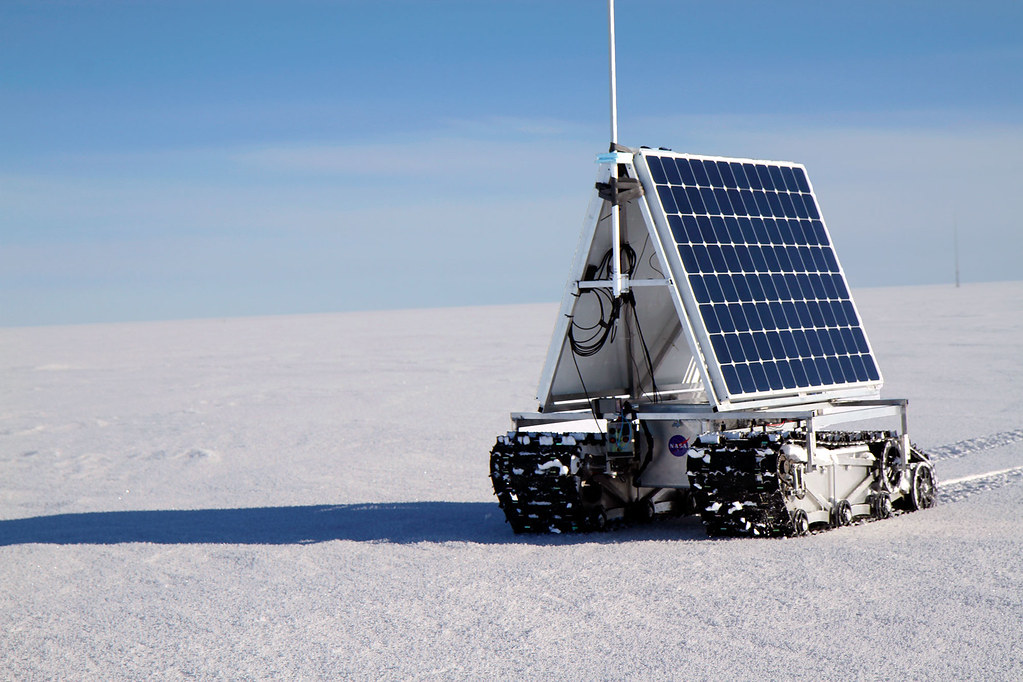
\includegraphics[width=0.5\linewidth]{\picPath/Cars/NasaGrover.jpg}
\end{center}
  \caption{  Гусеничный робот Nasa grover, разработанный для использования в условиях ледяной пустыни }
  \label{Figure:NasaGrover}
\end{figure}

Главный недостаток гусеничных роботов $-$ большая вариация возможных позиций робота после выполнения маневров. Маневрируя, гусеничный робот устанавливает скорость одного из гусеничных ходов отличной от другой, заставляя медленную гусеницу скользить по поверхности. В зависимости от типа поверхности и её состояния, положение робота после маневра может сильно варьироваться[Книжка], поэтому точное определение положения гусеничного робота затруднительно. Этот факт затрудняет построение автономного гусеничного робота. Кроме того, большая площадь пятна касания дает большее сопротивление качению, что замедляет робота. Большое количество элементов, содержащееся в гусеничном ходу, подвержено износу и имеет меньший запас прочности, чем обычное колесо. 

Гусеничный ход - компромис в пользу проходимости робота по пересеченной местности. Несмотря на все недостатки, гусеничные роботы широко в качестве боевых[ Публикации журнала "Специальная Техника" №6 1999 год.БАТАНОВ Александр Фёдорович
ГРИЦЫНИН Сергей Николаевич
МУРКИН Сергей Владимирович].
\end{document}